\begin{frame}{Motivation/Issues}
  \begin{itemize}
    \item Need to be able to accurately represent the confidence we should have in a model's prediction in the presence of all uncertainties--including uncertainty due to model inadequacy.
    \item In representing uncertainty due to model error, need to incorporate knowledge about the model and its weaknesses, e.g. constraints that must be respected, or approximations and omission in the formulation.
\item We will explore these issues in the context of models for contaminant
  dispersion in a porous medium
  \end{itemize}
\end{frame}

\begin{frame}{Addressing Model Inadequacy}
  \vspace{-1em}
  \begin{align*}
    0 &= \mathcal{R}( c, \tau; s )\\
    d &= \mathcal{O}(c, \tau; s ) + \epsilon_{obs}\\
    q &= \mathcal{Q}(c, \tau; s )
  \end{align*}
  \vspace{-1em}
  \begin{itemize}
    \item $\mathcal{R}$ - reliable theory, e.g. conservation laws.\vspace{-.5em}
    \item $\mathcal{O}$ - observation operator.\vspace{-.5em}
    \item $\mathcal{Q}$ - Q.o.I. mapping. \vspace{-.5em}
    \item $s$ - scenario parameters, e.g. BCs, physical constants\vspace{-.5em}
    \item $\tau$ - unknown quantities needed to solve for the state.
  \end{itemize}
    These equations are exact, but $\tau$ is unknown. The constitutive model $\tau\approx\tau_m(\theta)$ is introduced to close the equations.
\end{frame}

\begin{frame}{Addressing Model Inadequacy}
Represent the modeling error where it occurs, i.e. with the introduction of a constitutive model.
\begin{align*}
  \tau = \tau_m( \theta ) + \epsilon_{model}
\end{align*}
\begin{align*}
  0 &= \mathcal{R}(c, \tau_m + \epsilon_{model}; s)\\
  d &= \mathcal{O}(c, \tau_m + \epsilon_{model}; s ) + \epsilon_{obs} \\
  q &= \mathcal{Q}(c, \tau_m + \epsilon_{model}; s )
  \end{align*}
  Advantages over Kennedy \& O'Hagan formulation:
  \begin{itemize}
    \item Can propagate uncertainty in $\tau_m$ to the Q.o.I.
    \item Can respect what is known about $\tau$ and the deficiencies of $\tau_m$.
    \item Can respect physical constraints.
  \end{itemize}
\end{frame}

\begin{frame}{ \large Application to a Simple Contaminant Transport Problem}
  For a 1D model of contaminant transport in a porous medium, conservation of concentration is our reliable theory.
  \begin{align*}
    \mathcal{R}(c, q_{dispersion}; s) &= \diffp{c}{t} + \diffp{}{x}\cdot( uc + q_{dispersion} ) = 0, \\
    s &= [ u; c(0,t) = c(1,t); c(x,0) = c_0(t) ]
  \end{align*}
  A typical closure model for $q_{dispersion}$ is Fick's first law.
  Fick's first law is an inadequate representation of dispersion through a heterogeneous porous medium.
  So include an inadequacy model satisfying constraints.
  \begin{align*}
    &q_{dispersion} = -\nu \diffp{c}{x} + \epsilon_m(c)\\
    0 &= \mathcal{R}(c, \tau_m + \epsilon_m; s ) = \diffp{c}{t} + u \diffp{c}{x} +   \diffp{}{x}\left( -\nu \diffp{c}{x} + \epsilon_m(c) \right)
  \end{align*}
\end{frame}

\begin{frame}{ Model Error Representation }
  How to represent $\epsilon_{model}$ is an open problem.
  To guide its development we outline the basic requirements we have for the error representation.
  It should
  \begin{itemize}
    \item be stochastic, to represent the uncertainty we have in our model form;
    \item not violate physical constraints such as conservation laws and known characteristics of the state such as smoothness, positivity, etc.
  \end{itemize}
  Two approaches being pursued at PECOS are:
  \begin{itemize}
    \item Describe its behavior via a PDE describing its transport, generation, advection, etc. with random forcing.
    \item Represent it as a stochastic operator acting on the state variable.
  \end{itemize}

\end{frame}

\begin{frame}{ Calibrating a deterministic operator}
To test this idea we begin by first calibrating a deterministic operator.
  We define $\epsilon_m = \mathcal{L}(c)$ a linear, translation-invariant operator.
 \begin{align*}
  0 &= \mathcal{R}(c, \tau_m + \epsilon_m; s ) = \diffp{c}{t} + u \diffp{c}{x} +   \diffp{}{x}\left( -\nu \diffp{c}{x} + \mathcal{L}(c) \right)
  \end{align*}
Translation-invariant operators have fourier modes for eigenfunctions, i.e.
\begin{align*}
\mathcal{L}( e^{i2\pi kx} ) = \lambda_k e^{ i2\pi k x }.
\end{align*}
Only need to find the eigenvalues. How to constrain them?  Define priors to express our knowledge re. the form of $\mu_k$
\begin{align*}
	\mu_k &= r_k e^{i\theta_k}, \quad
	r_k \sim \mathcal{U}( 2 \pi k, ( 2\pi k )^{2} ), \quad \theta_k \sim \mathcal{U}( \pi/2, 3\pi/2 )
\end{align*}
\end{frame}

\begin{frame}{Problem dimensionality}
Although this is an infinite-dimensional problem, only a subset of the eigenvalues are informed by the data.
\begin{align*}
	c(x,t) = \sum_{k=-\infty}^{\infty} \widehat{c}(t)e^{i2\pi k x} \approx \sum_{k=-N/2}^{N/2} \widehat{c}(t)e^{i2\pi k x}
\end{align*}
For our problem, the dimension of the calibration problem went from $N=150$ to $13-15$.
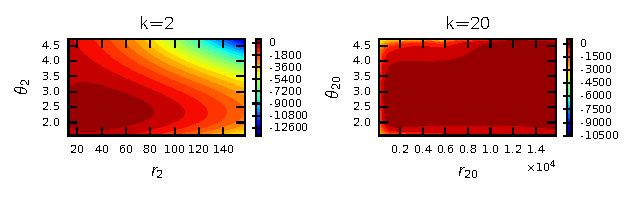
\includegraphics{rawfigs/fixedInconsistentExample/figs/presentation_log_lhoods.pdf}
\end{frame}

\begin{frame}{\large Inference - multiple sample locations, one time observation}
  \vspace{0.075\textheight}
  We calibrate the eigenvalues with MMALA in MIT'S UQ package (MUQ), seeding from the MAP point.
  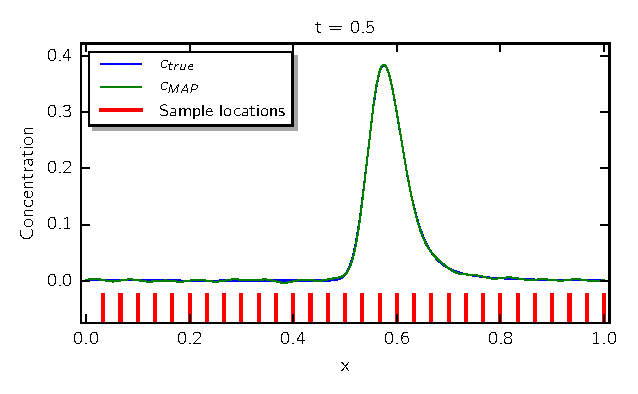
\includegraphics{{rawfigs/independentObservationsInSpace/figs/x_solution_t_0.5}.pdf}
\end{frame}

\begin{frame}{\large Posteriors - multiple sample locations, one time observation}
  \vspace{ .075\textheight}
  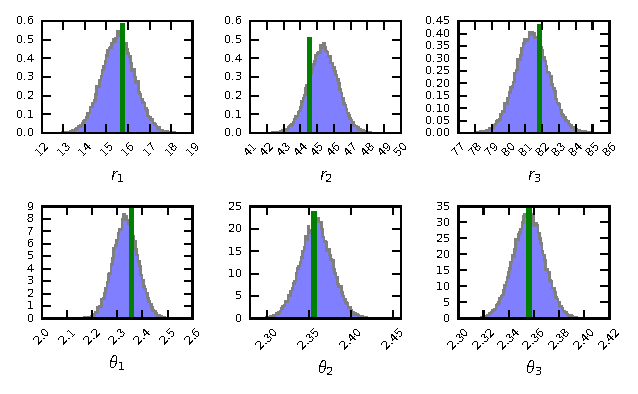
\includegraphics{rawfigs/independentObservationsInSpace/figs/presentation_histograms.pdf}
\end{frame}
